% Author: Andrew Hughes

\chapter{Algebraic Process Calculi}
\label{apc}

In this chapter, we focus on concurrency from a theoretical
perspective and introduce one of the main algebraic models for
modelling concurrent systems.  The topics and ideas discussed here lay
the foundations for the calculi we will discuss in chapters
\ref{globsync} and \ref{mobility}, and, as a result, are of great
importance in understanding the novel work presented in chapters
\ref{nt}, \ref{tnt} and \ref{dynamite}.

Early computational models took a simple idealised view of the world,
where events occur sequentially and in isolation.  Such a model is the
universal Turing machine \cite{turing:36} which has proven to be
computationally complete; it is capable of simulating all recursive
functions.  However, it does not directly model concurrent execution.

If a model can have this level of computational power without
attempting to represent concurrent behaviour, why is it necessary to
model concurrency at all?  Even though a method of modelling phenomena
exists, and has a certain level of expressivity, it doesn't imply that
it is the most appropriate for a particular context.  The existence of
both Turing machines and the $\lambda$ calculus already demonstrates
this point.  While both have proven equivalent in power, they take
different approaches to achieving this.

To see the effect of concurrency on computation, consider a simple
prototypical example, as demonstrated by Milner \cite{milner:lecture}.
Observe the following programs,

\begin{align*}
\mathtt{x} & \mathtt{= 2;}\tag{P1} \\
\\
\mathtt{x} & \mathtt{= 1;}\notag \\
\mathtt{x} & \mathtt{= x + 1;}\tag{P2}
\end{align*}

\noindent where we assume that each line is an atomic
action\footnote{This is a simplification; for example, \texttt{x = x +
    1} actually involves three atomic actions - reading the value of
  x, computing the value of x plus one and writing the result to x}.

In a sequential system, such as may be modelled by a Turing machine or the
$\lambda$ calculus, both these programs set \texttt{x} to 2.  In such a
system, there is only a single flow of control, so nothing else can
modify the value of \texttt{x}.

However, in a concurrent system, multiple control flows or processes
exist, each running in parallel with the others.  With P1, the value
of \texttt{x} will always be equal to two immediately after execution,
as the assignment takes place within a single atomic action.  However,
in P2, another process is free to modify \texttt{x} \footnote{Assuming
  \texttt{x} is accessible by more than one process.} between the
assignment of the value 1 and the later summation which makes
\texttt{x} 2.

Thus, if P2 is run in parallel with a third program,

\begin{equation}
\mathtt{x = 3;} \tag{P3}
\end{equation}

\noindent then \texttt{x} may end up being either 2, 3 or 4, depending
on whether P3 executes before the first line, after the completion of
P2, or after the first line respectively.  With P1 and P3, only 2 or 3
can result (which one depends on the order the two programs are run).
This is known as a \emph{race condition}, as the final value of
\texttt{x} depends on the timing of the various modifications of its
value by the two programs.  The solution to this problem is to require
each program to obtain exclusive access to \texttt{x} (a lock) for the
extent of its use.

This example demonstrates that modelling concurrency is not so much
about multiple programs executing at the same time, but instead
concerns how they interact.  If each program exists in its own
isolated environment and doesn't access any common resources, then no
interactions will take place and a sequential model for each would be
suitable.  Indeed, this is the way most operating systems handle
running multiple programs.  Thus, it follows that sequential models
are not distinct from concurrent models, but a subset where this
additional restriction of isolation applies.

Dijkstra's classic `Dining Philosophers' problem
\cite{dijkstra:philosophers} illustrates further issues which may
arise in a situation where multiple processes must interact to achieve
their goal.  In this scenario, five philosophers are seated around a
table, each with a plate of spaghetti and a fork.  The philosophers
divide their time between thinking and eating.  In order to eat, a
philosopher must obtain two forks, necessitating some form of
interaction.  This is a common situation in concurrency, where
multiple parallel processes (the philosophers) need to gain access to
a limited resource (the forks).

In cases where things go awry, \emph{deadlock} or \emph{starvation}
may result.  For example, if all the philosophers simultaneously pick
up the forks on their left, then none of them will be able to eat;
they will all end up waiting on a fork held by another philosopher.
The system is said to be \emph{deadlocked}, as none of the processes
can obtain a lock on the resource it needs, as a lock is already held
by one of the other processes\footnote{The solution to breaking this
  deadlock is to break the symmetry; if the fifth philosopher tries to
  take the fork on the right first, he or she will be unable to
  proceed, but the first philosopher will, using the fifth
  philosopher's left fork.}.  Alternatively, \emph{starvation} may
result (literally in this case) if one of the philosophers never stops
eating and consequently never releases the forks; the resources are
unfairly distributed to the deficit of one of the processes.

As can be seen from these examples, concurrency raises issues outside
the reach of traditional sequential models of computation.  Thus, just
as there is a requirement for models of sequential computation, models
that can represent these phenomena are also necessary.  This is even
more relevant today, as hardware advances make more machines capable
of true concurrency (via dual-core processors and beyond) and
distributed computing paradigms, such as services, become more
prevalent.  To adequately work with these systems, appropriate formal
models are needed to represent them and highlight their flaws.  Many
such models have been developed, and over the next three chapters, we
will consider a subset of these.

\section{The Calculus of Communicating Systems (CCS)}

Algebraic process calculi model the interaction of concurrent
processes using a (usually small) set of algebraic operators, as
opposed to the true concurrency of Mazurkiewicz trace theory
\cite{maz:trace} or the graphical style associated with Petri nets
\cite{petri:phd} and Hewitt's Actor model \cite{hewitt:actor}.
Interaction between processes is via message-passing, rather than via
shared memory\footnote{Although shared memory and message-passing are
  not orthogonal; a shared memory space may be represented as a
  communicating resource in a message-passing system, while message
  queues can be implemented in shared memory.} or a tuple space
\cite{linda}.

The foundational calculi in this field are Hoare's CSP \cite{hoare:csp78},
Milner's CCS \cite{milner:ccs} and Bergstra and Klop's ACP \cite{acp}, all of
which were first developed in the late 1970s to early 1980s.  CSP was
originally developed as a programming language, with a relatively large
syntax, and later given a theoretical basis, following Milner's work on
CCS.  Both calculi have influenced each other, while starting out from
different perspectives (Milner's being more of a theoretical one).  ACP
shares many of the ideas of CCS, and can be regarded as an
`alternative formulation' \cite{acp}, using a similar set of operators
to achieve a different goal.

Here, the focus is on CCS, as it forms the basis for most of the other
calculi considered, including the $\pi$ calculus
\cite{picalctutorial} and CaSE \cite{CaSE}.  Of the three, CCS has the
most minimal syntax with additional features such as failure
(represented in both CSP and ACP) needing to be derived from or appended to
this core set.  From a theoretical perspective, this is advantageous, as
it makes reasoning over the calculus a simpler process, and, as will be
seen, adding further syntax to represent more features is a relatively
simple process.

\subsection{CCS}
\label{ccs}

In CCS, processes are modelled as terms ranged over by $E, F$.  These
process terms have the following syntax:

\begin{equation}
\label{ccssyntax}
  E, F\ ::=\ 
  0\ |\ 
  \alpha.E\ |\ 
  E\backslash\ a\ |\ 
  E\ +\ F\ |\ 
  (E\ |\ F)\ |\ 
  X\ |\ 
  \mu X.E\ |\ 
  E[f] 
\end{equation}

\noindent where $\alpha$, $a$ and $f$ are explained below.

Communication between processes is via the sending and receiving of
signals.  The internal behaviour of the processes is abstracted,
represented simply by the silent action $\tau$.  The full set of
actions, $Act = \mathcal{N} \cup \overline{\mathcal{N}} \cup
\{\tau\}$, is used to describe the behaviour of the concurrent system,
where $\mathcal{N}$ is an infinite set of names, and
$\overline{\mathcal{N}}$ is the corresponding set of co-names,
$\{\overline{a} | a \in \mathcal{N}\}$.  These names are usually used
to represent \emph{channels}, which the processes use to communicate.
Thus, $a.E$, where $a \in \mathcal{N}$, represents a process whose
first action is an input on the channel $a$, whereas $\overline{a}.E$
(where $\overline{a} \in \overline{\mathcal{N}}$) represents a process
which initially outputs on $a$.

The behaviour of a single process is thus defined as a sequence of
inputs, outputs and silent actions. This can be seen in the above
grammar, where $0$ represents the empty process, which exhibits no
behaviour, and $\alpha.E$ is the action prefix used for the limited
sequential composition of actions, where $\alpha \in Act$.

For communication to actually take place, two processes must
\emph{synchronize}; they must emit corresponding actions on the same
channel at the same time.  For this to occur, the two processes must be
running in parallel.  Parallel composition in CCS is represented by the
$|$ operator.  When two processes are composed in this way, they may
both perform their corresponding input and output actions
simultaneously, resulting in a $\tau$ action being emitted.

For instance, if $E$ is considered to be $a.0$ and $F$ to be
$\overline{a}.0$, then the process formed by the composition of these
two processes, $E|F$ may initially perform one of three actions, $a$,
$\overline{a}$ or $\tau$, to give three possible derivations:

\begin{enumerate}
\item $E\ |\ F \derives{a} 0|F$
\item $E\ |\ F \derives{\overline{a}} E|0$
\item $E\ |\ F \derives{\tau} 0|0$
\end{enumerate}

\begin{figure}  
  \centering
\[
\xy
(20,0)*{a.\nil \mid \overline{a}.\nil}="1";
(0,-15)*{a.\nil \mid \nil}="2";
(40,-15)*{\nil \mid \overline{a}.\nil}="3";
(20,-30)*{\nil \mid \nil}="4";
{\ar@/^2pc/^{a} "1";"3"};
{\ar@/_2pc/_{\overline{a}} "1";"2"};
{\ar@/^2pc/^{\overline{a}} "3";"4"};
{\ar@/_2pc/_{a} "2";"4"};
{\ar^{\tau} "1";"4"};
\endxy
\]
%  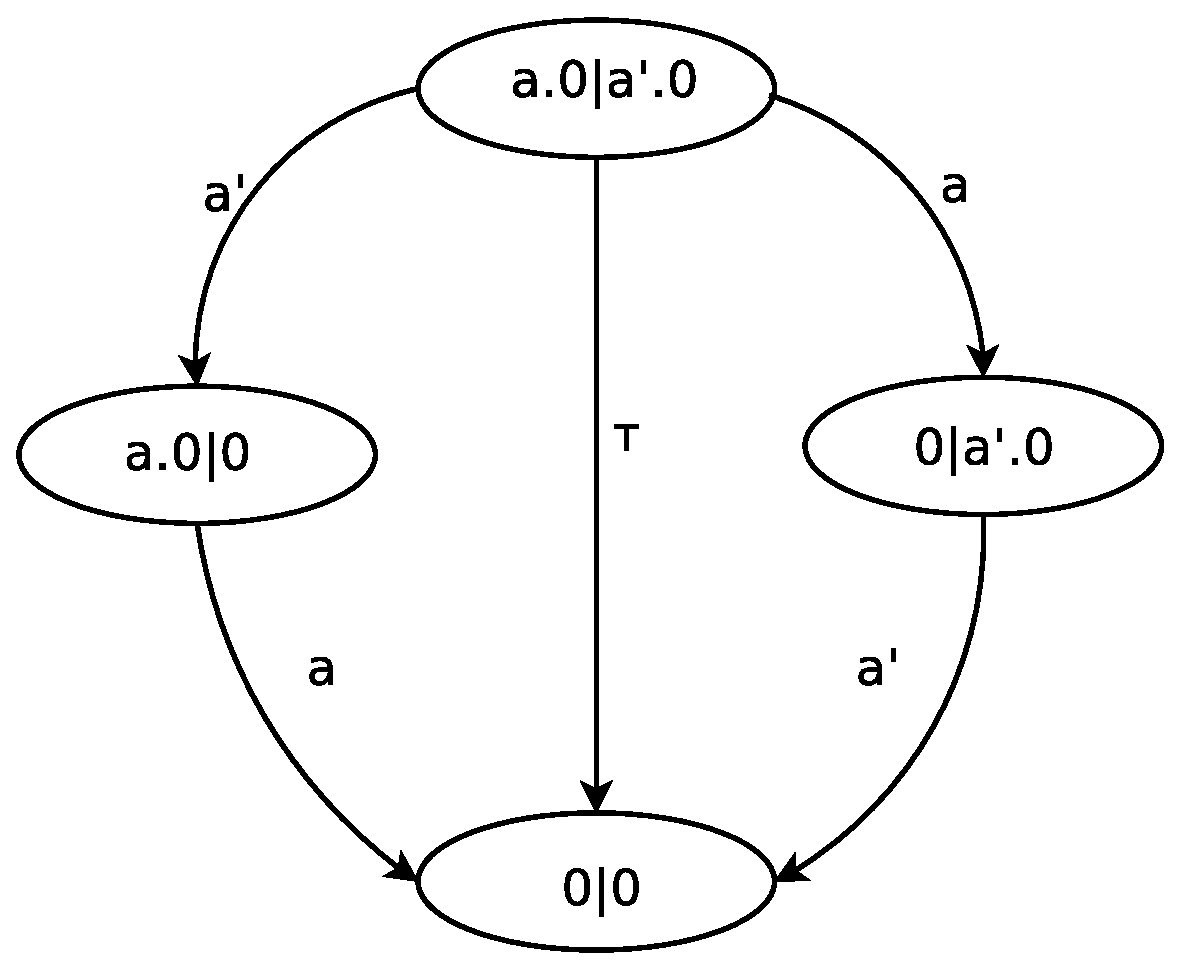
\includegraphics[scale=0.5]{graph1}
  \caption{Graph of $a.0 \mid \overline{a}.0$}
  \label{fig:graph1}
\end{figure}

This is illustrated in Fig. \ref{fig:graph1}.  To make the derivation
of $E|F$ deterministic, the scope of $a$ can be restricted.  In CCS,
an input or output can be paired with any corresponding action which
is within the scope of the channel.  To force the input of $E$ to be
paired with the output of $F$, the scope of $a$ must be restricted so
as to only include the two processes, $E$ and $F$.  This is handled by
another operator in the core syntax, $\backslash$.  The right operand
of this is the name of a channel whose scope is restricted to that of
the left operand.  In this case, $(E|F)\backslash a$ appropriately
limits the possible derivations to just $\derives{\tau}$.

The remaining binary CCS operator is $+$, which provides
non-deterministic choice between two processes.  Once a derivation is
made from one process, the option of performing the actions of the
other is lost.  This contrasts with the parallel composition operator,
where the other process remains running in parallel.  Choice thus
effectively corresponds to the familiar idea of branching found in
sequential models.  Using the same two exemplar processes again, $E +
F$ may derive as follows:

\begin{enumerate}
\item $E\ +\ F \derives{a} 0$
\item $E\ +\ F \derives{\overline{a}} 0$
\end{enumerate}


\begin{figure}  
  \centering
\[
\xy
(20,0)*{a.\nil + \overline{a}.\nil}="1";
(20,-30)*{\nil}="2";
{\ar@/^2pc/^{a} "1";"2"};
{\ar@/_2pc/_{\overline{a}} "1";"2"};
\endxy
\]
%  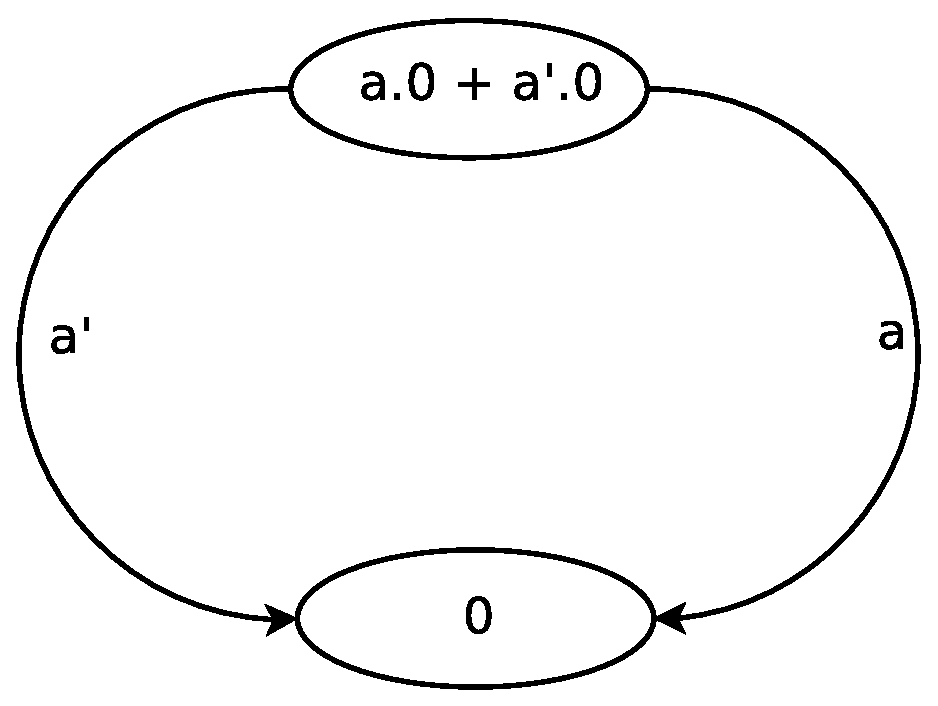
\includegraphics[scale=0.5]{graph2}
  \caption{Graph of $a.0 + \overline{a}.0$}
  \label{fig:graph2}
\end{figure}

Again, this is illustrated in Fig. \ref{fig:graph2}.  There are clearly
similarities between the two sets of possible derivations, but note
that, with choice, there is no possibility of synchronisation.

The remaining operators in CCS handle recursion and relabelling.  $\mu
X.E$ binds X with the value of $E$, so that later occurrences of $X$ are
replaced with $E$.  The function, $f$, in $E[f]$ has the type $Act
\rightarrow Act$ and converts actions, while preserving $\tau$ and
complementation.

\subsection{The Dining Philosophers in CCS}

To fully appreciate CCS, it is necessary to see how it may be used to
model an example scenario.  Consider the dining philosopher's example
illustrated above. Modelling this in CCS involves first ascertaining
what processes form the basis of this `system'.  Clearly, each
philosopher plays a part, so they should be represented by a process.
Returning to the original definition of the problem, each philosopher
may choose to eat or think.  In CCS, this can be represented as:

\begin{equation}
Philosopher = EatingPhilosopher\ +\ ThinkingPhilosopher
\end{equation}

\noindent where the philosopher is recursively defined as making the
choice between becoming an $EatingPhilosopher$ process or a
$ThinkingPhilosopher$ process.  Defining the latter is simple; 
thinking is simply some internal process of the philosopher:

\begin{equation}
ThinkingPhilosopher = \tau .Philosopher
\end{equation}

The focus of the model is on the eating process, which requires
access to the system's shared resource: the forks.  Modelling this
necessitates defining a protocol whereby the philosopher may interact
with the resource in order to obtain access to it.  From this, it
follows that the forks must also be represented as processes:

\begin{equation}
Fork = \mu X.takeFork.putDownFork.X
\end{equation}

\noindent with two communication channels, $takeFork$ and
$putDownFork$.  The fork begins its life on the table from which it
may be taken, represented here by the receipt of an input on the
$takeFork$ channel.  Once this has occurred, the process becomes
$Fork^\prime$,

\begin{equation}
Fork^\prime = putDownFork.X
\end{equation}

\noindent which represents the state where the fork is in use by a
philosopher.  The fork can't be used again until it has received an
input on $putDownFork$, which causes $X$ to be expanded and the fork to
wait for input on $takeFork$ again.

This interaction is further clarified by defining the final process,
the $EatingPhilosopher$:

\begin{equation}
EatingPhilosopher = \overline{takeFork}.\overline{takeFork}.\tau.\overline{putDownFork}.\overline{putDownFork}.Philosopher
\end{equation}

\noindent which needs to synchronize with two available $Fork$
processes to be able to eat (represented by $\tau$) and then release
the forks.  The system as a whole is modelled by running a number of
philosophers and forks in parallel (i.e. multiple copies of
Fig. \ref{fig:dpccs}), and restricting the scope of the fork channels
in order to enforce synchronisation.

\begin{figure}  
  \centering
  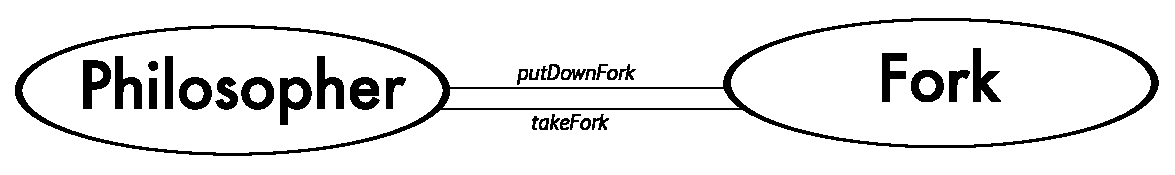
\includegraphics[scale=0.5]{philosophers}
  \caption{The Dining Philosophers in CCS}
  \label{fig:dpccs}
\end{figure}

Note that this CCS representation of the problem only models the
narrative version of the problem above.  There is no attempt to
resolve any of the competition problems, and a strong element of
non-determinism, as to which philosopher gets which fork, still
exists.  It does, however, give a formal representation of the problem
and allows the effects of varying the relative numbers of philosophers
and forks to be observed via execution of the model.

Modifying this slightly gives a model that corresponds
exactly to a specified number of philosophers and forks, $n$.  From
the definitions above, multiple variants may be generated, such that
each philosopher and fork process has a unique subscript.  For
example, $Philosopher$ becomes $Philosopher_i$, where $i = 1\dots n$.
The same subscripting also applies to the $takeFork$ and $putDownFork$
channels, so that they now correspond to a specific fork.  The
original solution can thus be represented, as the case where each
philosopher, $i$, initially performs the action $takeFork_i$ (to take
the left fork) and then $takeFork_{i-1}$ (with the exception that when
$i-1 = 0$, we use $n$) \footnote{Again, it is necessary to reverse the
  actions of $Philosopher_n$ in order to obtain a solution that does not
  deadlock.}.

This model restricts which fork is taken by which philosopher
(limiting the possible actions, and thus removing some
non-determinism), but is still prone to the effects of
non-deterministic choice (some philosophers may arbitrarily choose to
think instead) and fairness, with regards to action performance (if
the actions are performed in a depth-first manner, only one
philosopher may end up eating).  These may be regarded as
implementational aspects of the model; all these phenomena could be
represented, but a choice between these is not made at this level of
abstraction.

\subsection{Advantages and Limitations of CCS}
\label{ccslimit}

From its syntax, it is clear that CCS can model sequential behaviour
using sequential composition ($\alpha.E$), non-deterministic choice
($+$) and $\nil$.  This further confirms the intuition noted earlier that
sequential programs are a subset of the larger set of concurrent
programs.  This is illustrated by the $+$ operator, which
returns a smaller set of possible derivations, from the same initial
pair of processes, when compared with parallel composition ($|$).
These sequential operators can also be used to convert a set of
parallel-composed processes into their equivalent interleavings.

CCS can model both sequential and concurrent programs, while still
maintaining a minimal syntax.  However, the calculus is not
Turing-complete\footnote{A finite axiomatisation can be defined, if
  the simultaneous presence of parallel composition and recursion is
  avoided \cite{milner:ccsaxiom}.}; there are limitations as to what
may be expressed.  As discussed earlier, Turing completeness does not
necessarily guarantee the suitability of a model for a particular
task. Likewise, the lack of such completeness doesn't imply that the
model is unsuitable.  As shown above, an appropriate model of the
Dining Philosophers problem may be defined, without Turing
completeness.  The lack of this in CCS is not necessarily a problem.
It may even be an advantage in some cases, where this lack of
expressivity simplifies the formal reasoning over the model.

One fairly obvious limitation, and one that is relevant when
discussing Turing completeness, is that there is no data in the model.
The processes discussed so far don't explicitly communicate anything
when they send or receive signals.  Instead, behaviour arises purely
from synchronisation.  It is possible to extend CCS to represent this
by adding the concept of value passing between processes.  A host of
other process calculi have been based on such a variant of CCS, and we
will consider this in more detail as part of section \ref{mobility}.

CCS models are also relatively static; while processes may evolve
(e.g. $a.P$ may become $P$) and the number of processes in the system
may change (e.g. a process may branch using parallel composition), the
communication structure doesn't.  Notably, if a process, $E$ knows
about the channels $x$ and $y$ initially, while $F$ only knows about
$x$ (due to restriction on $y$), this status can not change during the
course of the various transitions inherent in the system.

The effect of restriction is more generally known as \emph{scoping}
and occurs frequently with reference to variables in programming
languages.  CCS doesn't allow dynamic changes to the scoping of
channels.  Instead, scoping is fixed to the static arrangement
provided by the initial system, prior to any transitions.  The
addition of dynamic scoping, often referred to as mobility, is the
major contribution of the $\pi$ calculus, a language based on CCS
covered in \ref{scopemobility}.

To conclude, there is another limitation of CCS which is less to do
with a particular concept being absent from the language, instead
being more related to its central aspect: \textbf{synchronisation}.
The problem here lies in the \emph{compositionality} of processes.
While the structure of a CCS system remains compositional, because the
result of parallel composition is determined by the behaviour of the
composed processes together with the rules of the $|$ operator, this
is not true of the synchronisation of multiple processes.

Consider the idea of broadcasting a signal to an arbitrary number of
processes.  Ideally, a general \emph{broadcast agent} should be
defined which provides this behaviour.  In CCS, there are at least two
possible ways of defining semantics for the agent, but not one that
provides a suitably compositional solution.  Perhaps the most obvious
of these is simply to extend the familiar synchronisation of two
processes.  An input and output pair can synchronize, so why not just
create multiple pairs, one for each receiving process?  For example,
transmitting a signal to two processes can be written simply as

\begin{equation}
\mathbf{\overline{a}_1.\overline{a}_2.0}\ |\ a_1.P\ |\ a_2.Q
\end{equation}

\noindent where the process on the left (in bold) forms the semantics
for the broadcast agent and the processes, $P$ and $Q$ are the
continuations of the input processes

This will work, but what happens when the broadcast agent needs to
transmit the signal to three processes?

\begin{equation}
\mathbf{\overline{a}_1.\overline{a}_2.\overline{a}_3.0}\ |\ a_1.P\ |\ a_2.Q\ |\ a_3.R
\end{equation}

\noindent The semantics of the broadcast agent have to change.  Simply
composing the third input will lead to one of the three being ignored
by the original definition of the broadcaster given above.  So, simply
enumerating multiple synchronisation pairs is not sufficient to
provide a compositional broadcast agent.

A second solution lies in recursion.  If the problem with the previous
solution lies in the broadcasting agent doing too little (i.e. not
transmitting to all the possible receivers), then, by making it
recurse, it will keep sending the output to whoever will synchronize
with it.  Thus, the example for three inputs above becomes

\begin{equation}
\mu X.\overline{o}.X\ |\ o.P\ |\ o.Q\ |\ o.R
\end{equation}

\noindent which works, and will continue to do so if a further
input process is parallel composed.  

But there is still a problem for much the same reasons as the first
solution.  This works fine on this small scale, but what happens when
this agent is placed in the context of a larger system?  Once the agent
starts its cycle of outputs, it won't stop as there exists
no base case for this recursion\footnote{A base case may be introduced
using non-deterministic choice, but there is no guarantee when this will
be invoked, if ever.}.  An output on $o$ will always be available (within
the scope of any restriction placed on that particular channel) and
the broadcasting process can never do anything else.  The result is a
constantly cycling process, which, in an implementation of this model,
would continue to consume resources.

The true solution to this problem is to enable some form of
\emph{global synchronisation}.  This requires a separate entity,
disparate from the processes involved in the communication, which can
be used to co-ordinate the synchronisation.  In the next section, a
branch of process calculi is considered which provides just such a facility.

\section{Conclusion}

In conclusion, this review has taken a brief look at the field of
concurrency, largely from the perspective of process calculi.
Initially, it was shown that, while universal Turing machines and the
$\lambda$ calculus can simulate any recursive function, their inherent
sequential behaviour makes them unsuitable for modelling concurrent
systems.  CCS, in contrast, is less expressive but can model this kind
of behaviour.





